\usepackage{tikz}
\usetikzlibrary{positioning,calc,external}

\title{ITC8280 Fundamentals of Cryptography}
\subtitle{TLS, CT and CAA}
\date{\today}
\author{Taaniel Kraavi}
\institute%
{%
  \textit{School of Information Technologies}\\
  \textit{Tallinn University of Technology}
}

\begin{document}
\begin{frame}
  \titlepage
\end{frame}

\begin{frame}{Securing traffic on the web}
  How do we create a secure communication channel over a network?

  \vspace*{1em}

  \pause
  What do we protect against?
  \begin{itemize}[<+(1)->]
    \item Eavesdropping
    \begin{itemize}
      \item $\implies$ Confidentiality
    \end{itemize}
    \item Tampering
    \begin{itemize}
      \item $\implies$ Integrity \& authenticity
      \item Integrity must be authenticated (accidental vs. malicious modifications)
    \end{itemize}
    \item Impersonation/forgery
    \begin{itemize}
      \item $\implies$ Authenticity
    \end{itemize}
  \end{itemize}

  \vspace*{1em}

  \pause
  We need a \emph{protocol} satisfying these requirements.
\end{frame}

\begin{frame}{SSL \& TLS}
  Secure Sockets Layer (SSL) by Netscape
  \begin{itemize}[<+(1)->]
    \item SSL 1.0 never released (security flaws)
    \item SSL 2.0 (1995) deprecated in 2011 (\href{https://datatracker.ietf.org/doc/html/rfc6176}{RFC 6176})
    \item SSL 3.0 (1996) deprecated in 2015 (\href{https://datatracker.ietf.org/doc/html/rfc7568}{RFC 7568}) 
  \end{itemize}

  \vspace*{1em}

  \pause
  Transport Layer Security (TLS)
  \begin{itemize}[<+(1)->]
    \item Born out of SSL 3.0 with interop.-breaking changes
    \item TLS 1.0 (1999) \& TLS 1.1 (2006), deprecated in 2021 (\href{https://datatracker.ietf.org/doc/html/rfc8996}{RFC 8996})
    \item TLS 1.2 (2008, \href{https://datatracker.ietf.org/doc/html/rfc5246}{RFC 5246}) not yet deprecated, but should
    \item TLS 1.3 (2018, \href{https://datatracker.ietf.org/doc/html/rfc8446}{RFC 8446}) obsoletes RFC 5246
  \end{itemize}
\end{frame}

\begin{frame}{Transport Layer Security (TLS)}
  TLS is a cryptographic \emph{protocol}.
  \begin{itemize}[<+(1)->]
    \item Used for securing HTTPS, email, VoIP, instant messaging, \dots
    \item Assumes a reliable transport protocol (e.g. TCP)
    \par
    \begin{itemize}
      \item Datagram TLS (DTLS) for unreliable transport (e.g. UDP)
    \end{itemize}
    \item TLS 1.3 is designed following formal security models
  \end{itemize}

  \vspace*{1em}

  \pause
  Connections are negotiated with the \emph{TLS handshake}.
  \begin{itemize}[<+(1)->]
    \item Parties agree upon and validate various parameters
    \item The subsequent \enquote{secure} connection is stateful
  \end{itemize}
\end{frame}

\begin{frame}{TLS handshake overview}
  The client and server agree on the following:
  \begin{itemize}[<+(1)->]
    \item TLS version to use (1.2 or 1.3)
    \begin{itemize}
      \item No support for older versions = no downgrade risk\textsuperscript{*}
    \end{itemize}
    \item Cipher suite to use
    \begin{itemize}
      \item Set of algorithms for establishing the secure connection
      \item Client and server agree on what they both support
    \end{itemize}
    \item Authenticate the server's identity
    \begin{itemize}
      \item Server's public key \& certificate chain\textsuperscript{*}
      \item Optionally also the client's identity: mutual TLS (mTLS)
    \end{itemize}
    \item Create session keys
    \begin{itemize}
      \item These protect the actual communication session
    \end{itemize}
  \end{itemize}
\end{frame}

\begin{frame}{TLS 1.3 handshake with DH}
  \begin{figure}
    \center
    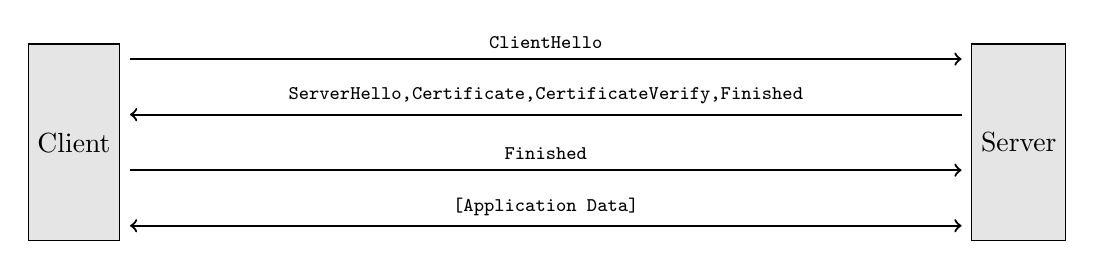
\begin{tikzpicture}
      \node[draw,minimum height=2.5cm,fill=gray!20] (client) at (0,0)   {Client};
      \node[draw,minimum height=2.5cm,fill=gray!20] (server) at (12, 0) {Server};

      \node (A) at (client.east) [yshift=30px] {};
      \node (B) at (server.west) [yshift=30px] {};
      \node (C) at (client.east) [yshift=10px] {};
      \node (D) at (server.west) [yshift=10px] {};
      \node (E) at (client.east) [yshift=-10px] {};
      \node (F) at (server.west) [yshift=-10px] {};
      \node (G) at (client.east) [yshift=-30px] {};
      \node (H) at (server.west) [yshift=-30px] {};

      \draw[->,thick]  (A) -- (B) node[midway,above] {\scriptsize\texttt{ClientHello}};
      \draw[<-,thick]  (C) -- (D) node[midway,above] {\scriptsize\texttt{ServerHello,Certificate,CertificateVerify,Finished}};
      \draw[->,thick]  (E) -- (F) node[midway,above] {\scriptsize\texttt{Finished}};
      \draw[<->,thick] (G) -- (H) node[midway,above] {\scriptsize\texttt{[Application Data]}};
    \end{tikzpicture}
  \end{figure}

  \begin{itemize}[<+(1)->]
    \item {\small\texttt{ClientHello}}: nonce, client's DH share, and supported parameters
    \item {\small\texttt{ServerHello}}: negotiated connection parameters, server's DH share
    \item {\small\texttt{Certificate}}: server's certificate (and the cert. chain)
    \item {\small\texttt{CertificateVerify}}: signature over the entire handshake
    \item {\small\texttt{Finished}}: MAC over the entire handshake (AEAD tag)
  \end{itemize}

  \pause
  Other variants exist (e.g. 0-RTT with a PSK, 2-RTT with HRR, mTLS).
\end{frame}

\begin{frame}{Improvements of TLS 1.3}
  \begin{itemize}[<+(1)->]
    \item Legacy symmetric encryption algorithms pruned
    \begin{itemize}
      \item Only AEAD schemes remain
    \end{itemize}
    \item De-facto inclusion of ECC, e.g.\ EdDSA
    \item Various crypto improvements
    \par
    \begin{itemize}
      \item RSA-PSS instead of PKCS\#1 v1.5
      \item Removed DSA, custom DHE groups \&  EC point compression
    \end{itemize}
    \item Static cipher suites removed
    \par
    \begin{itemize}
      \item Always has perfect forward secrecy (PFS)
      \item Exception: when only pre-shared keys (PSK) are used
    \end{itemize}
  \end{itemize}
\end{frame}

\begin{frame}{Perfect forward secrecy (PFS)}
  A hybrid problem:
  \begin{itemize}[<+(1)->]
    \item Servers have long-term keys, e.g. signing and encryption
    \item Client encrypts a symmetric key and sends it to the server (static RSA)
    \item If the server key is compromised, all previous shared keys could be recovered
  \end{itemize}

  \vspace*{1em}

  \pause
  PFS prevent past sessions from being decrypted if long-term keys leak.
  \begin{itemize}[<+(1)->]
    \item Generate a new key for each communication session (ephemeral key)
    \item Discard the keys after the session
    \item Only meaningful if the cryptosystem has not been broken
    \item TLS 1.3 always has PFS (except for PSK-only)
  \end{itemize}
\end{frame}

\begin{frame}{Quantum-safe handshake}
  PFS breaks if the key-confidentiality algorithm breaks.
  \begin{itemize}[<+(1)->]
    \item harvest-now/decrypt-later attacks
    \item \href{https://datatracker.ietf.org/doc/html/draft-ietf-tls-hybrid-design-16}{draft-ietf-tls-hybrid-design-16}
    \item Supported by OpenSSL since v3.5
    \par
    \begin{itemize}
      \item Prior to this, use e.g. the \href{https://github.com/open-quantum-safe/oqs-provider}{OpenQuantumSafe provider} for OpenSSL
    \end{itemize}
    \item Supported (and pushed by) CloudFlare
    \par
    \begin{itemize}
      \item Supported by Zone in Estonia
    \end{itemize}
    \item Handshake explained \href{https://www.ria.ee/blogi/tls-13-votme-kvantkindel-hubriidkehtestus-x25519mlkem768}{\textit{in Estonian}}, \href{https://blog.cloudflare.com/post-quantum-for-all/}{\textit{in English}}, \href{https://www.pqctoday.com/learn/tls-basics/}{\textit{\enquote{simulator}}}
  \end{itemize}

  \vspace*{1em}

  \pause
  Eventually we need quantum-safe certificates, but this is less urgent.
\end{frame}

\begin{frame}{Improvements of TLS 1.3 (cont.)}
  \begin{itemize}[<+(1)->]
    \item Encryption of handshake messages after the Server Hello
    \begin{itemize}
      \item Good for privacy, e.g. encrypted client certificate for mTLS
    \end{itemize}
    \item Simplified handshake in general
    \item Dropped renegotiation support
    \begin{itemize}
      \item New session must be established to change parameters
    \end{itemize}
    \item \dots
  \end{itemize}
\end{frame}

\begin{frame}{TLS 1.3 cipher suites}
  The TLS v1.3 RFC specifies 3 principal cipher suites:
  \pause
  \begin{itemize}
    \item {\small\texttt{TLS\_AES\_128\_GCM\_SHA256}} (must)
    \item {\small\texttt{TLS\_AES\_256\_GCM\_SHA384}} (should)
    \item {\small\texttt{TLS\_CHACHA20\_POLY1305\_SHA256}} (should)
  \end{itemize}

  \vspace*{1em}

  \pause
  Also specified, but often not enabled by default:
  \begin{itemize}
    \item {\small\texttt{TLS\_AES\_128\_CCM\_8\_SHA256}}
    \item {\small\texttt{TLS\_AES\_128\_CCM\_SHA256}}
  \end{itemize}
\end{frame}

\begin{frame}{TLS 1.2 cipher suites}
  TLS 1.2 specified 37 in the original RFC\dots
  \begin{itemize}
    \item Confusing nomenclature
    \item e.g. {\small\texttt{TLS\_ECDHE\_RSA\_WITH\_AES\_128\_GCM\_SHA256}}
  \end{itemize}
\end{frame}

\begin{frame}{Some resources}
  Checking TLS 1.3 support:
  \begin{itemize}
    \item {\small\url{https://caniuse.com/tls1-3}} for browser support
    \item \href{https://support.globalsign.com/ssl/general-ssl/tls-protocol-compatibility}{GlobalSign's reference}
    \item \href{https://learn.microsoft.com/en-us/windows/win32/secauthn/protocols-in-tls-ssl--schannel-ssp-}{Windows support table}
  \end{itemize}

  \pause
  Testing a website's configuration:
  \begin{itemize}
    \item {\small\url{https://www.ssllabs.com/ssltest/}}
    \item {\small\url{https://www.hardenize.com}}
  \end{itemize}

  \pause
  Some cipher suite recommendations (for TLS 1.2 support)
  \begin{itemize}
    \item \href{https://developers.cloudflare.com/ssl/reference/cipher-suites/recommendations/}{Cloudflare recommendations}
    \item \href{https://www.iana.org/assignments/tls-parameters/tls-parameters.xhtml?ref=hackernoon.com\#tls-parameters-4}{IANA recommendations}
  \end{itemize}
\end{frame}

\begin{frame}{Root programs}
  \pause
  Which CAs to trust by default?
  \begin{itemize}[<+(1)->]
    \item \href{https://aka.ms/RootCert}{Microsoft Trusted Root Program}
    \item \href{https://www.apple.com/certificateauthority/ca_program.html}{Apple Root Certificate Program}
    \item \href{https://wiki.mozilla.org/CA}{Mozilla's CA Certificate Program}
    \item \href{https://g.co/chrome/root-policy}{Chrome Root Program}
    \item \dots
  \end{itemize}
\end{frame}

\begin{frame}{Some CAs}
  Popular CAs for TLS certificates:
  \begin{itemize}[<+(1)->]
    \item Let's Encrypt\textsuperscript{*}
    \item \href{https://www.globalsign.com/en}{GlobalSign}
    \item \href{https://www.sectigo.com}{Sectigo}
    \item \href{https://www.digicert.com}{DigiCert}
    \item \href{https://www.actalis.com}{Actalis}
  \end{itemize}
  
  \vfill

  \pause
  Market share yearly trends for TLS certificate authorities:

  {\scriptsize\url{https://w3techs.com/technologies/history_overview/ssl_certificate/ms/y}}
\end{frame}

\begin{frame}{Web certificate types}
  Domain validated (DV)
  \begin{itemize}[<+(1)->]
    \item Proof of control over WhoIS records
    \item Typical confirmation: HTTP challenge, DNS record, email contact\textsuperscript{*}
    \item Free these days (e.g. Let's Encrypt)
  \end{itemize}

  \pause
  Organisation validated (OV)
  \begin{itemize}[<+(1)->]
    \item Verification of org's name and registration status
  \end{itemize}

  \pause
  Extended validated (EV)
  \begin{itemize}[<+(1)->]
    \item Selected CAs, verification of legal identities, physical presence, \dots
    \item {\scriptsize\url{https://cabforum.org/working-groups/server/extended-validation/documents/}}
  \end{itemize}

  \pause
  Menu options instead of address bar distinction in modern browsers.
\end{frame}

\begin{frame}{Let's Encrypt}
  \pause
  \textit{Let's Encrypt is a free, automated, and open certificate authority brought to you by the nonprofit Internet Security Research Group (ISRG).} ({\scriptsize\url{https://letsencrypt.org}})
  \begin{itemize}[<+(1)->]
    \item Provides DV TLS certificates to any compatible client
    \begin{itemize}
      \item Verifies domain ownership via unique tokens
      \item Tokens validated with HTTP/DNS requests
    \end{itemize}
    \item Automated using ACME (Automatic Certificate Management Environment)
    \item \href{https://certbot.eff.org}{Certbot}
    \begin{itemize}
      \item Convenient ACME client
      \item Automatic TLS configuration on Nginx/Apache
      \item Other ACME clients exist
    \end{itemize}
  \end{itemize}

  \pause
  No excuse to have a non-HTTPS website.
\end{frame}

\begin{frame}{Browsers and active revocation}
  Browsers often skip revocation checks due to connectivity, performance, and privacy reasons.

  \vspace*{1em}

  \pause
  In \href{https://cabforum.org/2023/07/14/ballot-sc063v4-make-ocsp-optional-require-crls-and-incentivize-automation/}{2023}, the CA/B forum made CRLs mandatory, and OCSP optional for TLS certificates.
  \begin{itemize}[<+(1)->]
    \item Some CAs, including Let's Encrypt, dropped OCSP support as a result
  \end{itemize}
\end{frame}

\begin{frame}{Browsers and active revocation}
  Chrome-based:
  \begin{itemize}[<+(1)->]
    \item OCSP staples are checked, but no live OCSP checks
    \item \href{https://www.chromium.org/Home/chromium-security/crlsets/}{CRLSets} contain \enquote{important} revocations
  \end{itemize}

  \vspace*{1em}

  \pause
  Firefox:
  \begin{itemize}[<+(1)->]
    \item Staples are checked, but no live checks for DV-certificates (since FF 142)
    \item \href{https://hacks.mozilla.org/2025/08/crlite-fast-private-and-comprehensive-certificate-revocation-checking-in-firefox/}{CRLite}, comprehensive(-ish) CRL using efficient lookup (since FF 137)
    \par
    \begin{itemize}
      \item \href{https://wiki.mozilla.org/CA/Revocation_Checking_in_Firefox\#OneCRL}{OneCRL}: older solution, revoked intermediate and high-profile leaf certificates
    \end{itemize}
  \end{itemize}

  \vspace*{1em}

  \pause
  Apple does some weird OS-level revocation aggregation, which extends to Safari.
\end{frame}

\begin{frame}{TLS certificate lifetimes}
  Instead of active revocation, automation and short-lived certificates are the future.
  \begin{itemize}
    \item CA/B ballot \href{https://cabforum.org/2025/04/11/ballot-sc081v3-introduce-schedule-of-reducing-validity-and-data-reuse-periods/}{SC081v3}, April 2025
  \end{itemize}

  \vspace*{1em}

  \pause
  The maximum TLS certificate lifetime is:
  \begin{itemize}
    \item 200 days as of March 15, 2026
    \item 100 days as of March 15, 2027
    \item 47 days as of March 15, 2029
    \par
    \begin{itemize}[<+(1)->]
      \item Domain validation data may only be reused for 10 days
    \end{itemize}
  \end{itemize}
\end{frame}

\begin{frame}{Certificate transparency (CT)}
  Certificate transparency (\href{https://datatracker.ietf.org/doc/html/rfc9162}{RFC 9162}) helps us identify mis-issued certificates.
  \begin{itemize}[<+(1)->]
    \item Public log of certificates issued by trusted CAs
    \par
    \begin{itemize}
      \item Append-only logs
      \item Operated by browser vendors and CAs themselves
    \end{itemize}
    \item Signed certificate timestamp (SCT)
    \begin{itemize}
      \item Signed by another log operator within a maximal delay
      \item Browsers require SCT for publicly trusted TLS certificates
    \end{itemize}
    \item Monitor your domains to check for unapproved issuance
    \begin{itemize}
      \item {\scriptsize{\url{https://certificate.transparency.dev/monitors/}}}
      \item {\scriptsize{\url{https://crt.sh}}}
    \end{itemize}
  \end{itemize}
\end{frame}

\begin{frame}{Certificate pinning}
  Certificates and keys can be \emph{pinned}.
  \begin{itemize}[<+(1)->]
    \item Client device contains a list of approved certificates
    \par
    \begin{itemize}
      \item e.g. Estonian i-voting client (I think)
    \end{itemize}
    \item \enquote{Precursor} to certificate transparency
    \par
    \begin{itemize}
      \item HTTP Public Key Pinning -- HTTP header with public key hashes
      \item Obsoleted in favour of CT
    \end{itemize}
    \item Generally not practical:
    \par
    \begin{itemize}
      \item Lack of flexibility and scalability
      \item Complex and risky (e.g. DoS in case of issues)
    \end{itemize}
  \end{itemize}

  \pause
  Pinning typically invites more trouble than it is worth.
\end{frame}

\begin{frame}{Certification Authority Authorization (CAA)}
  CAA (\href{https://datatracker.ietf.org/doc/html/rfc8659}{RFC 8659}) is a type of DNS record that lets us specify:
  \begin{itemize}[<+(1)->]
    \item which CAs can issue certificates for our domain,
    \item what methods they can use to confirm control over the domain.
  \end{itemize}

  \vspace*{0.5em}

  \pause
  Compliant CAs must not issue certificates when not in the allowlist.
  \begin{itemize}[<+(1)->]
    \item Mitigates malicious requests to compliant CAs
    \item Not retroactive: checked only during issuing
    \item Relying parties (e.g. browser) must not use CAA info for validation
  \end{itemize}

  \vspace*{0.5em}

  \pause
  CAA is a fail-safe complement to CT, but not a necessity.
\end{frame}

\begin{frame}{SSL stripping}
  MITM attacks can undermine proper HTTPS configurations.

  \vspace*{1em}

  \pause
  SSL stripping (HTTP downgrade) attacks:
  \begin{enumerate}[<+(1)->]
    \item Intercept a user's initial HTTP request (before HTTPS upgrade/redirect)
    \item Establish an HTTPS session with the server
    \item Serve the site to the user over HTTP
    \item Steal the user-provided data
  \end{enumerate}
\end{frame}

\begin{frame}{HTTP Strict Transport Security (HSTS)}
  HSTS helps prevent SSL stripping attacks.

  \pause
  An HSTS policy:
  \begin{itemize}[<+(1)->]
    \item Specifies that only HTTPS access should be used (during a period)
    \item Requires trust on first use (TOFU) for the client to store the preference
    \item HSTS preloading avoids TOFU ({\small\url{https://hstspreload.org}})
  \end{itemize}

  \vspace*{1em}

  \pause
  Similar logic to the OCSP Must-Staple certificate extension.
  \begin{itemize}[<+(1)->]
    \item Similar risks too: DoS if misconfigured
    \item Unlike OCSP stapling, you should use HSTS on your websites
  \end{itemize}
\end{frame}

\begin{frame}{A glimpse into the timeline}
  \begin{center}
    \url{https://www.feistyduck.com/ssl-tls-and-pki-history/}
  \end{center}
\end{frame}

\end{document}
